\chapter{循环神经网络加速技术基础}

\section{循环神经网络及其变体}
循环神经网络是一种专门针对序列数据进行建模的神经网络模型。有别于前馈神经网络,卷积神经网络等“静态模型”,循环神经网络在结构上拥有循环
自连接的反馈机制,这使得模型当前的输出不仅取决于当前输入,还与当前的状态有关。通过对状态的存储与更新,循环神经网络能够有效的建模动态系统。
理论上,任何图灵可计算的函数都可以用有限维的循环网络近似。尽管循环神经网络功能强大,但是高昂的训练成本阻碍了循环神经网络的实际应用。
一方面,固定有序的前向传播过程只能遵循序列顺序先后计算,因此通过时间的反向传播无法并行计算;另一方面,梯度消失和梯度爆炸问题在循环神经网络
的训练过程中尤为突出,这导致其学习长期依赖关系变的困难。随着理论研究的发展和算力的提升,以上问题都得以解决。借助第三次人工智能浪潮
循环神经网络重新焕发出勃勃生机,目前,循环神经网络已经广泛应用于自然语言处理等相关领域。

\subsection{普通循环神经网络}
普通循环神经网络是最简单的循环神经网络结构,主要包括输入层,隐藏层和输出层。输入层对输入进行特征提取并映射为固定长度的向量,隐藏层将输入信息
和前一时刻的状态转化为新的状态,输出层根据网络存储的状态解码并完成输出。其中隐藏层包含记忆信息以及记忆更新的规则,是循环神经网络中最重要的
结构。
常见的循环神经网络结构如图\ref{fig:rnn}所示,权重矩阵\(U, W, V\)分别表示输入到到隐藏,隐藏到隐藏,隐藏到输出之间的连接,向量\(x, h, o\)分别表示输入单元,
隐藏单元和输出单元,这些单元及其相互连接形成网络。相比于其他网络模型的单向信息传递,循环神经网络引入环状结构实现了从输入到输出的双向信息
流动。一些符合训练准则的信息将会通过循环的方式长期保存在网络状态中,并根据输入序列特征进行适时唤醒记忆。当网络记忆的信息足够丰富时,循环神经
网络不仅能准确的预测输出,并且能大致恢复输入序列。自编码器框架就是基于此原理而产生,其能根据记忆的状态信息选择重要的输入并近似复制到输出,
实现特征学习或降维。图中左侧为循环神经网络回路原理图,黑色方块表示回路中单个时间步的延迟,即时刻t-1的状态会影响时刻t的状态。图中右侧为
循环神经网络按时间展开的计算图,展开是指将左侧的回路结构映射为右侧的包含重复组件的结构,展开的深度取决与序列的长度。循环神经网络展开结构图
显式的数据流动路径描述了信息是如何在时间上向前和向后传递的。
\begin{figure}
	\centering
	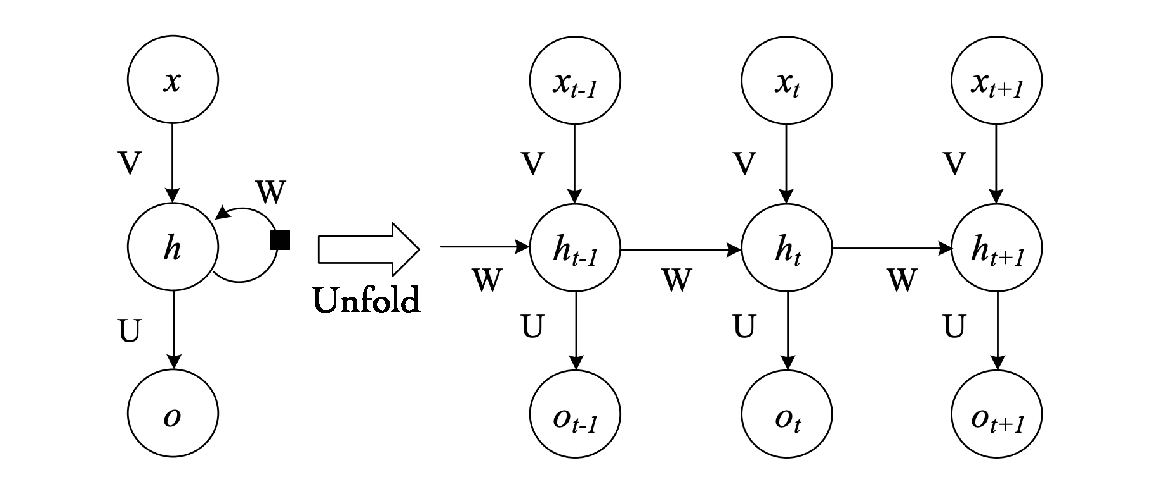
\includegraphics[width=0.8\columnwidth]{RNN_struct.eps}
	\caption{普通循化神经网络结构图}
	\label{fig:rnn}
\end{figure}

循环神经网络的数学模型为式\ref{eq:rnn}, 其中\(g\), \(f\)分别表示隐藏层和输出层的激活函数。在循环神经网络中\(g\)一般选用\(sigmoid\),\(tanh\)
等饱和性激活函数以避免训练过程中可能出现的梯度爆炸问题。函数表达式除了描述模型输入与输出的关系外,还规定了循环神经网络内部结构的
一般特性:

(1)状态的长度固定,即模型的记忆容量有限。\(h_t\)作为过去序列与任务相关方面的有损摘要,只能根据训练准则选择性的保留过去序列的某些方面特质。

(2)模型单个时间步的输入是固定的。无论序列的长度,模型每个时刻始终具有相同大小的输入,状态转移也只能从一种状态转移到下一种状态,
而不是在可变长度的输入序列或历史状态上进行操作。

(3)每个时间步使用相同参数的相同转移函数,即输出的每一项是对先前输出应用相同的更新规则而产生的。更新规则在时间上共享,模型能够表示序列间的相互影响。
相比在所有时间步均建立独立的学习模型,单一的共享模型在非训练集的序列上具有良好的泛化能力。

\begin{equation}\label{eq:rnn}
	\begin{split}
		h_{t} &= g(W*h_{t-1} + U*x_{t})	\\
		y_{t} &= f(V*h_{t})						
	\end{split}
\end{equation}

循环神经网络的训练采用通过时间的反向传播算法(Back-propagation through time,BPTT)。梯度计算首先将一段序列依次送入模型进行前向传播,
保存前向传播过程中的各个状态并计算最终的损失函数;然后,计算梯度并沿时间反向更新权重参数。由于循环网络的计算涉及相同函数的多次组合,
无论沿时间正向或者反向,当需要捕获的依赖关系需要跨越很长的时间尺度时,输入和输出会出现极端的非线性行为。具体的,如果雅可比矩阵的最大特征值
小于1,多次连乘后梯度会趋于0,梯度消失会使得模型参数无法更新,梯度下降算法永远不会收敛到最优解;如果雅可比矩阵的最大特征值大于1,那么随着
时间跨度的增大,梯度也将越来越大,最终会导致权重剧烈改变,学习也变得不稳定。梯度消失和梯度爆炸问题使得循环神经网络学习序列的长期依赖
关系变得困难, 目前,研究人员提出了一些降低学习长期依赖难度的方法,在某些情况下循环神经网络可以学习跨越百步的依赖关系,尽管取得了很大的进步
但是,如何学习更长时间的依赖关系仍然是深度学习领域的一个主要挑战。


\subsection{长短期记忆神经网络}
长短期记忆神经网络(Long short-term memory,LSTM)是目前应用范围最广的一种循环神经网络,相比简单的循环架构,LSTM能更容易的学习到长期依赖。
其结构中存在多层循环,除了外部的循环外,内部还存在“LSTM细胞”自循环。多层循环使得时间路径增加,梯度消失的可能性被大大降低,因此更深的循环神经
网络架构也得以实现\citing{}。

LSTM网络结构如图\ref{fig:lstm}所示,输入信息需要经过多条数据路径并进行复杂的加工处理才能最终到达隐藏层,这些位于数据路径中的“门”控制着信息的通过率。
其值越接近1表示该信息越需要被记忆,越接近0表示信息应该迅速被丢弃。通过控制信息的通过率,网络能够在较长的时间内持续积累线索,并且尽量少的受
干扰信息影响,因此累积的时间尺度可以动态的调节。LSTM网络中的门主要包括输入门\(i\),遗忘门\(f\)和和输出门\(o\),网络的输入信息包括细胞态\(c_{t-1}\),
状态\(h_{t-1}\)以及输入\(x_t\)。

在LSTM网络的前向传播过程中,首先当前的输入\(x_t\)和上一时刻的状态\(h_{t-1}\)会共同生成遗忘门的通过率,上一时刻的细胞态\(c_{t-1}\)会在此门
的控制下选择性的通过。然后,在输入门的控制下,输入信息中的重要线索会被合并到新的细胞状态中。最后细胞当前的状态会通过输出门进行最终的
筛选并产生新的状态。以上输入信息和记忆信息在三个门控单元的层层作用下,序列中符合学习经验的信息将会在很长的时间尺度内被收集起来,实现长期记忆,
而无关的信息所形成的短期记忆则会随着时间流逝迅速被遗忘。

LSTM网络的数学模型为式\ref{eq:lstm},


\begin{figure}
	\centering
	\includegraphics[width=1\columnwidth]{LSTM_struct.eps}
	\caption{LSTM结构图}
	\label{fig:lstm}
\end{figure}


\begin{equation}\label{eq:lstm}
	\begin{split}
		&i_t = \sigma(W_{ix}*x_t + W_{ir}*h_{t-1} + b_i)	\\
		&f_t = \sigma(W_{fx}*x_t + W_{fr}*h_{t-1} + b_f)	\\
		&g_t = \sigma(W_{cx}*x_t + W_{cr}*h_{t-1} + b_c)					\\
		&c_t = f_t \odot c_{t-1} + g_t \odot i_t							\\	
		&o_t = \sigma(W_{ox}*x_{t} + W_{or} * h_{t-1} + b_o)	\\
		&m_t = o_t \odot h_{c_t}											\\
		&h_t = W_{hm}*m_t													
	\end{split}
\end{equation}


\subsection{回声状态网络} 

\section{模型压缩与加速算法}
RWG 基函数是定义在三角形单元上的最具代表性的基函数。它的具体定义如下:
\begin{equation}
f_n(\bm{r})=
\begin{cases}
\frac{l_n}{2A_n^+}\bm{\rho}_n^+=\frac{l_n}{2A_n^+}(\bm{r}-\bm{r}_+)&\bm{r}\in T_n^+\\
\frac{l_n}{2A_n^-}\bm{\rho}_n^-=\frac{l_n}{2A_n^-}(\bm{r}_--\bm{r})&\bm{r}\in T_n^-\\
0&\text{otherwise}
\end{cases}
\end{equation}

其中,$l_n$为三角形单元$T_n^+$和$T_n^-$公共边的长度,$A_n^+$和$A_n^-$分别为三角形单元$T_n^+$和$T_n^-$的面积(如图\ref{pica}所示)。

\begin{figure}[h]
	\includegraphics{pica.pdf}
	\caption{RWG 基函数几何参数示意图}
	\label{pica}
\end{figure}

由于时域混合场积分方程是时域电场积分方程与时域磁场积分方程的线性组合,因此时域混合场积分方程时间步进算法的阻抗矩阵特征与时域电场积分方程时间步进算法的阻抗矩阵特征相同。
\begin{equation}
\label{latent_binary_variable}
\bm{r}_{i,j}=
\begin{cases}
1,f(\bm{x}^{i};\bm{w})\cdot f(\bm{x}^{j};\bm{w})\geq u(\lambda),\\
0,f(\bm{x}^{i};\bm{w})\cdot f(\bm{x}^{j};\bm{w})< l(\lambda), 1\leq i,j\leq n.\\
f(\bm{x}^{i};\bm{w})\cdot f(\bm{x}^{j};\bm{w}),\text{otherwise},
\end{cases}
\end{equation}

时域积分方程时间步进算法的阻抗元素直接影响算法的后时稳定性,因此阻抗元素的计算是算法的关键之一,采用精度高效的方法计算时域阻抗元素是时域积分方程时间步进算法研究的重点之一。


\subsection{轻量化网络}

\subsection{模型稀疏化}

\subsection{数值量化}

\subsection{张量分解}

\section{硬件加速平台介绍}

\subsection{FPGA硬件加速技术}

\subsection{开发工具}


如图\ref{picb}和图\ref{picc}所示分别给出了参数$E_0=\hat{x}$,$a_n=-\hat{z}$,$f_0=250MHz$,$f_w=50MHz$,$t_w=4.2\sigma$时,调制高斯脉冲的时域与频域归一化波形图。

\begin{figure}[h]
\subfloat[]{
	\label{picb}
	\includegraphics[width=7.3cm]{picb.pdf}
}
\subfloat[]{
	\label{picc}
	\includegraphics[width=6.41cm]{picc.pdf}
}
\caption{调制高斯脉冲时域与频率波形,时域阻抗元素的存储技术也是时间步进算法并行化的关键技术之一。(a)调制高斯脉冲信号的时域波形;(b)调制高斯脉冲信号的频域波形}
\label{fig1}
\end{figure}

时域阻抗元素的存储技术\citing{xiao2012yi}也是时间步进算法并行化的关键技术之一,采用合适的阻抗元素存储方式可以很大的提高并行时间步进算法的计算效率。

\section{本章小结}
本章首先从时域麦克斯韦方程组出发推导得到了时域电场、磁场以及混合场积分方程。

